% !Mode:: "TeX:UTF-8"
\documentclass{xcumcmart}
\usepackage{setspace}
\usepackage{enumerate}
\usepackage{tabu}
\usepackage{listings}
\usepackage{color}
\usepackage{graphicx}

\definecolor{dkgreen}{rgb}{0,0.6,0}
\definecolor{gray}{rgb}{0.5,0.5,0.5}
\definecolor{mauve}{rgb}{0.58,0,0.82}

\lstset{frame=tb,
  language=Python,
  aboveskip=3mm,
  belowskip=3mm,
  showstringspaces=false,
  columns=flexible,
  basicstyle={\small\ttfamily},
  numbers=none,
  numberstyle=\tiny\color{gray},
  keywordstyle=\color{blue},
  commentstyle=\color{dkgreen},
  stringstyle=\color{mauve},
  breaklines=true,
  breakatwhitespace=true,
  tabsize=3
}
% \title{text}这里是显示在第三页的文章标题
\title{基于线性模型的钢水“脱氧合金化”方案优化}
\linespread{1.2} %行距
\begin{document}
\renewcommand\arraystretch{2}

\maketitle
\begin{cnabstract}%此处没有采用sbstract命名,是为了将来如果要加入英文摘要时扩展的方便
\setlength{\parskip}{1.4em} %段落距离

\par 本文针对HRB400B这一特定型号的钢材,探讨了对钢水脱氧合金化过程中对C,Mn,Si,S,P这五种元素含量的影响因素,使用线性回归模型,用于对添加合金料的自动配比并在保证钢材主要元素含量指标合格的情况下实现成本控制。
\par 问题一中,本文针对C和Mn这两种元素,利用公式计算两种元素的收得率。针对影响因素,本文采用相关系数作为判定标准,进行定性分析,再对数据归一化处理并使用线性回归模型进行定量分析,发现收得率的影响因素主要为钢水净重和加入的元素含量、转炉终点中的原有元素含量。
\par 问题二中,需要对Mn和C这两种元素的收得率进行预测。在进行离群值、缺失值等预处理后,以转炉终点成分的含量以及钢水净重,温度,添加的合金料的量等因素作为自变量,将C和Mn的吸收率作为结果,尝试了决策树模型,线性模型,贝叶斯模型进行拟合,并使用多个回归模型评价指标进行综合评价。其中由于贝叶斯模型和线性模型在该问题上的拟合程度较高,考虑到数据的特点,本文最终选用了线性模型用于拟合,并取得了较好的结果。
\par 对于问题三,加入了C,Mn,Si,P,S这五个元素含量的限制条件,同时也加入了合金料的价格因素以拟合钢水脱氢化的成本。本文针对钢水脱氢化成本的优化问题,首先沿用了第二问的线性预测模型,并针对HRB400B型号钢材建立配料优化方案,根据其元素含量标准建立线性约束不等式,再根据配料价格建立价格目标函数,使用线性规划进行优化,得到最优配料成本为551元每吨。
\par \textbf{关键词:脱氧合金化 线性回归 回归模型评价指标 线性规划}
\end{cnabstract}

\setlength{\parskip}{1.4em}
\setcounter{tocdepth}{2}
\setlength{\parskip}{1em} %段落距离
\tableofcontents
\newpage%增加目录,要不要都可以。不想要的话,就在本行前加“%”(英文的百分号)
\setlength{\parskip}{1.4em} %段落距离
\section{问题重述}
\par 目前,各大钢铁企业为提高竞争力所要解决的重要问题是:如何在保证钢水质量的同时最大限度降低合金钢的生产成本。这要求我们通过历史数据对脱氧合金化环节建立数学模型,在线预测并优化投入合金的种类及数量,最终实现成本-收益最大化目标。我们需要通过题目所给数据解决如下问题:
\begin{enumerate}[(a)]%(\arabic{section}.1)
\setlength{\itemindent}{2em}    %标签缩进量
\item 计算C、Mn两种元素的历史收得率,并分析影响其收得率的主要因素。
\item 基于问题1,对C、Mn元素收得率进行预测,并对模型进行改进。
\item 基于问题2实现钢水脱氧合金化的成本优化计算,并给出合金配料方案。
\item 根据研究结果给炼钢厂提出建议。
\end{enumerate}

\section{问题分析}
\par 题目需要我们通过对合金钢的生产历史数据进行分析,应该利用统计学知识以及数据处理的方法,对数据进行适当的预处理,再根据题目的具体要求,利用合理的指标和算法进行建模,并进行模型检验。
\par 问题一要求我们根据历史数据测算出C、Mn两种元素的历史收得率。计算之前应对数据的缺失情况进行分析,并合理地进行缺失值按行或按列丢弃、均值替代等操作,保证计算的可靠性。针对收得率影响因素的研究,首先使用相关系数进行定性的初步判定,其次增加线性回归进行定量分析。
\par 问题二要求我们对收得率进行预测,并改进模型及算法提高预测的准确性。第一题线性模型可以实现对元素收得率的预测,在此基础上模型改进有以下两点:第一,进一步确定元素收得率在实际工业应用中的可能影响因素,考虑数据缺失情况以及预测模型的需要,处理缺失值较多的变量时,将转炉终点缺失值替换为均值,重新计算收得率;第二,使用多种回归算法,通过合理的回归评价指标确定最佳模型算法。
\par 问题三是目标函数最优化问题,利用第二问的预测模型稍加修改,可实现对连铸合金的元素含量预测,根据题目所给HRB400B型号合金钢的元素含量标准建立线性约束,由于仅需要优化配料的成本,将未知的转炉终点元素含量以及转炉终点温度、钢水质量等无关变量全部使用均值替代,最终建立价格目标函数求解满足条件的最优方案。
\par 问题四则为基于上述问题的分析结果提出本团队的生产建议。

\section{假设与符号}
\subsection{假设条件}
\begin{enumerate}[(1)]
\item 除了附件数据中给定的条件外,如生产设备,操作步骤和生产工艺等一致。
\item 附件中脱氧合金化所给反应数据与化学反应时间无关,及所有反应时间相同或达到化学平衡状态。
\item 本题附件中提供的数据符合真实情况,钢材生产过程中没有其他人为因素的影响。
\item C、Mn等元素的收得率仅与题目所给数据项相关,即忽略其他可能存在的潜在影响。
\end{enumerate}


\subsection{符号说明}
\begin{table}[htbp]
	\centering
	\begin{tabu}{l l}
		\tabucline[1.5pt]{-}
		符号 & 说明\\
		\tabucline[1.5pt]{-}
		$\mu$ & 某组数据的平均值\\
		$\sigma$ & 某组数据的标准差\\
		$R_x$ & 元素x在某种化合物配料中的含量\\
		$X$ & 所有可能影响合金元素收得率的因素的值构成的向量,例如转炉温度、合金配料的质量等\\
		$f(x)$ & 生产单位质量HRN400B所需配料的成本\\
		$Y$ & 元素收得率或连铸正样中元素的含量\\
		\tabucline[1.5pt]{-}
	\end{tabu}
	\caption{符号说明\label{tb:fuhao}}
\end{table}

\section{问题一的解答}
\subsection{问题一的分析}
\par 由题目可得,合金收得率是指脱氧合金化时被钢水吸收的合金元素的重量与加入 该元素总重量之比。转炉终点指脱氧合金化之前钢水中某个元素的含量,连铸正样为脱氧合金化之后钢水中该元素的含量,因而被吸收的合金元素重量可用连铸正样与转炉终点的差值表示,再除以加入的该元素总重量即可求得历史收得率。通过分别分析各变量与C、Mn之间的相关系数初步判断合金收得率的影响因素,其次通过构建线性回归与归一化进行定量分析,最终得出收得率的影响因素。
\subsection{数据描述与预处理}
\par 附件一中的数据主要包括转炉终点各元素含量、连铸正样各元素含量以及加入合金配料质量、钢水总质量等数据项。
\par 部分变量的缺失值较多,例如:C、Mn元素连铸正样只有906组历史采样数据。因此将未采样的连铸正样数据行丢弃。
\par 如图\ref{fig:prev},通过直方图和折线图可以看到数据中存在离群值,且数据大致呈正态分布,为了提高分析的可靠性,需要将离群值去掉,仅保留$[\mu-3\sigma,\mu-3\sigma]$范围类的数据,根据正态分布3$\sigma$原则,该范围理论上包括99.73\%的原始数据。
\begin{figure}[htbp]
	\centering
	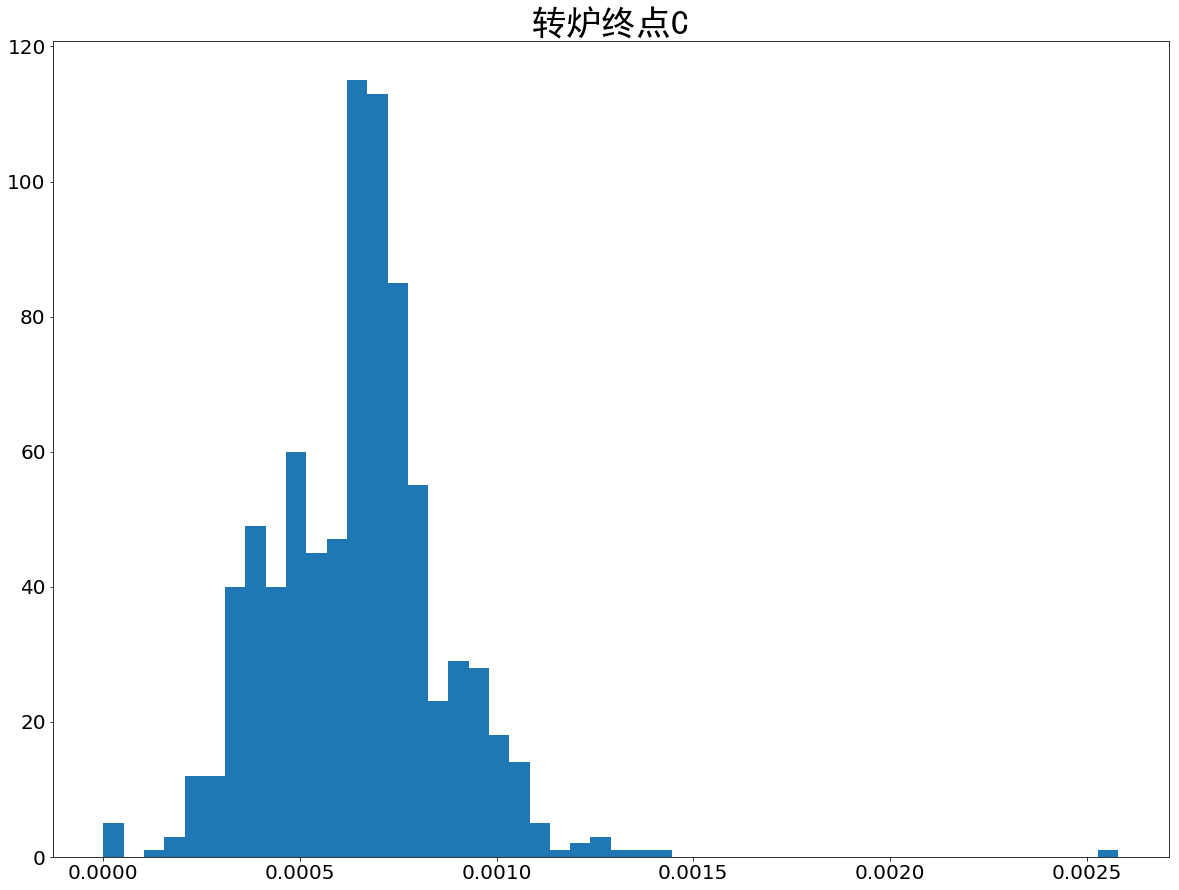
\includegraphics[width=0.45\textwidth]{fig/hist.png}
	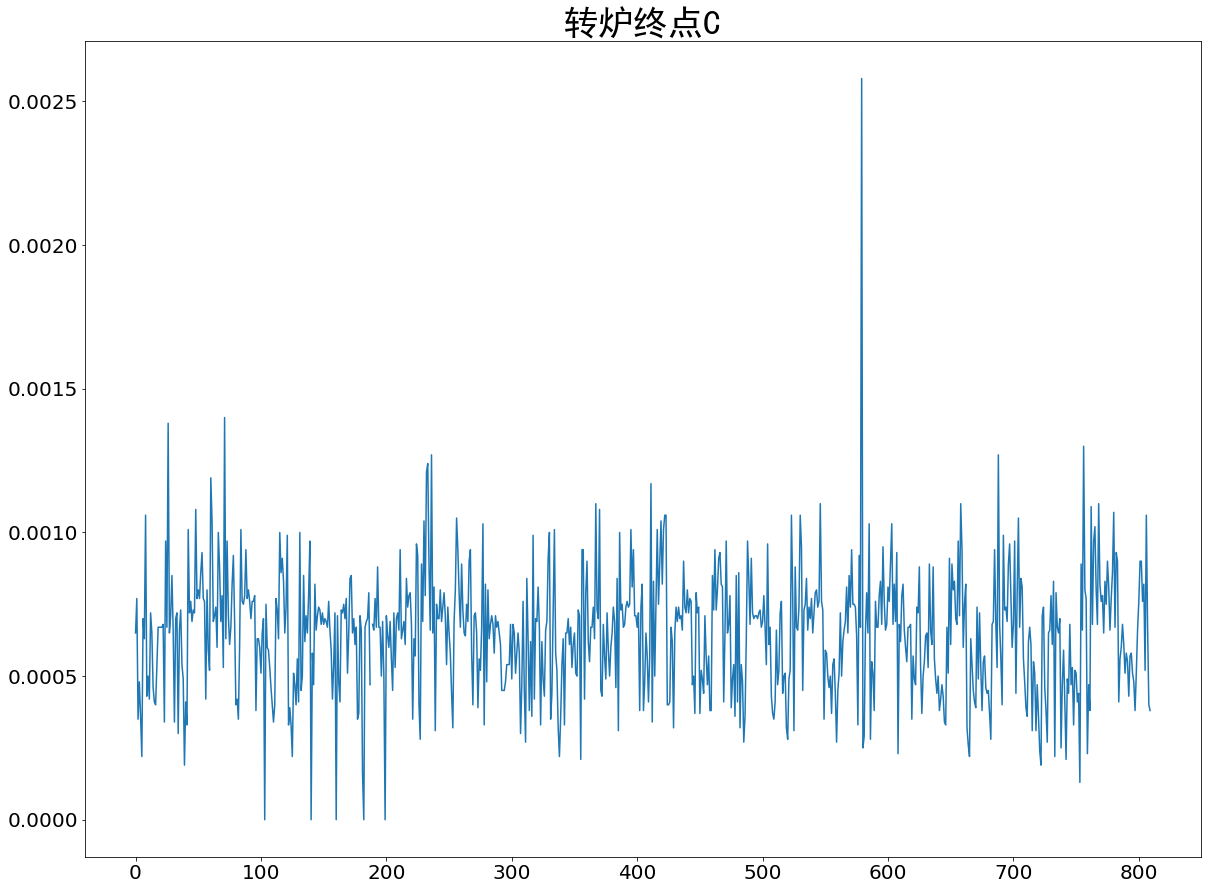
\includegraphics[width=0.45\textwidth]{fig/index.png}
	\caption{转炉终点C的数据分布\label{fig:prev}}
\end{figure}
\subsection{历史收得率的计算}
由题目可得,合金历史收得率的计算公式为:
\begin{equation} \label{eq:eps1}
    H_i=\frac{M(Out_i-Beg_i)}{T_i}\times 100\%
\end{equation}
  其中,$T_i$为添加配料中元素i的总质量,计算方式为$T_i=C_{i}^{T}X$,$X$为加入配料的质量构成的向量,$C_i$为每种配料对应元素i的含量。
$Beg_i$、$Out_i$分别为脱氧合金化前后钢水中元素i的含量。计算得到的历史收得率见附录。

\subsection{使用相关系数进行影响因素分析}
相关系数(Correlation coefficient)是反应变量之间关系密切程度的统计指标,相关系数的取值区间在1到-1之间。1表示两个变量完全线性相关,-1表示两个变量完全负相关,0表示两个变量不相关。数据越趋近于0表示相关关系越弱。公式\ref{eq:eps2}是相关系数的计算公式:
\begin{equation} \label{eq:eps2}
    r_{xy}=S_{xy}/(S_xS_y )
\end{equation}

其中$r_{xy}$ 表示样本相关系数,$S_{xy}$ 表示样本协方差,$S_x$ 表示$x$的样本标准差,$S_y$  表示$y$的样本标准差。下面分别是$S_{xy}$协方差和$S_x$和$S_y$标准差的计算公式。由于是样本协方差和样本标准差,因此分母使用的是$n-1$。
\[S_{xy}=\frac{\sum{i=1}^n(X_i-\overline{X})(Y_i-\overline{Y})}{n-1}\]
\[S_x=\sqrt{\frac{(X_i-\overline{X})^2}{n-1}}\]
\[S_y=\sqrt{\frac{(Y_i-\overline{Y})^2}{n-1}}\]

\par 我们分别计算了脱氧合金化过程中与C、Mn两种元素相关的变量与该元素收得率之间的相关系数,并保留了相关系数绝对值大于0.1的影
响因素,C、Mn相关系数见表\ref{tb:tbs1}、\ref{tb:tbs2}:
\begin{table}[htbp]
	\centering
	\begin{tabu}{l l}
		\tabucline[1.5pt]{-}
		影响因素 & C收得率\\
		\tabucline[1.5pt]{-}
		转炉终点C & -0.2888\\
		钢水净重 & 0.5026\\
		低铝硅铁 &0.4112\\
		石油焦增碳剂 & -0.2685\\
		\tabucline[1.5pt]{-}
	\end{tabu}
	\caption{C收得率与主要影响因素的相关系数\label{tb:tbs1}}
\end{table}
\begin{table}[htbp]
	\centering
	\begin{tabu}{l l}
		\\
		\tabucline[1.5pt]{-}
		影响因素 & Mn收得率\\
		\tabucline[1.5pt]{-}
		碳化硅(55\%) &-0.2163\\
		钒铁(FeV50-B).1 & -0.1861\\
		钒氮合金(进口) & 0.2486\\
		低铝硅铁 &	0.9407\\
		钢水净重 &	0.9440\\
		\tabucline[1.5pt]{-}
	\end{tabu}
	\caption{Mn收得率与主要影响因素的相关系数\label{tb:tbs2}}
\end{table}
\par 根据表\ref{tb:tbs1},C元素历史收得率的影响因素主要为C元素的转炉终点含量(脱氧合金化之前钢水中相应元素含量)、钢水净重、低铝硅铁、石油焦增碳剂。钢水净重与低铝硅铁于C元素的历史收得率呈正相关,钢水净重的影响表明钢水质量增加可以吸收更多的合金元素,转炉终点C和石油焦增碳剂对C元素历史收得率均有不同程度的负向响,表明加入过量的C化合物将导致C的收得率降低。根据表\ref{tb:tbs2},钢水净重、低硅铝铁和钒氮合金总体对Mn收得率有正向的影响,碳化硅和钒铁(FeV50-B)的加入更有可能使Mn收得率减小。
\begin{table}[htbp]
	\centering
	\begin{tabu}{l l |l l}
		\tabucline[1.5pt]{-}
		影响因素 & 回归系数 & 影响因素 & 回归系数\\
		\tabucline[1.5pt]{-}
		转炉终点温度  &  -0.0429 &  硅钙碳脱氧剂  &  -0.0158\\
		转炉终点C  &  -0.7986  &  转炉终点S  &  0.0012\\
		钢水净重  &  0.1989  &  氮化钒铁FeV55N11-A  &  -0.0468\\
		碳化硅(55\%)  &  -0.3568  &  钒氮合金(进口)  &  -0.0743\\
		钒铁(FeV50-A)  &  -0.0311  &  钒铁(FeV50-B)  &  -0.0\\
		钒铁(FeV50-B).1  &  -0.0276  &  硅铝钙  &  0.047\\
		硅铝合金FeAl30Si25  &  0.0545  &  硅铝锰合金球  &  0.0\\
		硅锰面(硅锰渣)  &  -0.0277  &  硅铁(合格块)  &  -0.0379\\
		硅铁FeSi75-B  &  -0.0449  &  石油焦增碳剂  &  -1.1481\\
		锰硅合金FeMn64Si27(合格块)  &  -0.1487  &  锰硅合金FeMn68Si18(合格块)  &  -0.2989\\
		\tabucline[1.5pt]{-}
	\end{tabu}
	\caption{C收得率线性回归模型对应系数\label{tb:tbs3}}
\end{table}

\subsection{使用线性回归进行影响因素分析}
\par 为了定量判断影响因素,首先进行数据的归一化处理,进而构建线性模型,从而可以通过模型的参数确定各影响因素及其影响程度。构建如式\ref{eq:esp3}线性模型:
\begin{equation}\label{eq:esp3}
	Y=\sum_{i=1}^na_iX_i+\varepsilon , \quad i=1,2,3,\ldots ,n
\end{equation}
其中$Y$为元素收得率,$X$为与该元素有关的影响因素,$a$为回归系数,表明该影响因素对元素收得率的影响程度,$n$为可能的影响因素数目,即加入合金配料的种类数,$\varepsilon$为偏差。

\par 对C收得率进行线性回归拟合,得到系数矩阵$[a_i]$及其对应变量如表\ref{tb:tbs3}。由于影响因素的变量数据经过了归一化,表中的回归系数大小可以定量的描述各个因素对C收得率的相对影响,钢水净重对元素收得率影响程度最大,且为较强的正相关关系,其次为C元素的转炉终点,二者具有较强的负相关关系;则更加石油焦增碳剂、锰硅合金、碳化硅(55\%)等的含量则会明显降低C元素的收得率,而增加硅铝钙的含量则会提高收得率。



\section{问题二的解答}
\subsection{问题二的分析}
\par 本问题是预测C, Mn的收得率,自变量为转炉终点各元素的含量,温度,钢水重量以及添加材料的量等.
\par 在问题1的基础上,本团队对预测模型进行了两点改进,第一,将变量中的缺失值用均值替代,这样可以增加用于训练的样本量以提升拟合的准确度。第二,C、Mn元素的初始含量较低,和连铸正样中相应元素的含量有着指数级的差距,对反应收得率的影响较小。在建立模型的时候,为了简化计算步骤,可以使用均值替代,或者直接舍去这些因素。第二,除了使用线性回归之外,本团队还尝试构建多种非线性模型来进行不同方案间的比较,例如:决策树回归、SVM(支持向量机)、贝叶斯回归、集成回归、多项式回归等,以提高预测收得率准确性。



\subsection{数据预处理}
\begin{enumerate}[(a)]
\setlength{\itemindent}{2em}    %标签缩进量
\item 对数据进行离群值的去除处理,仅保留$[\mu-3\sigma,\mu-3\sigma]$范围内的数据,根据正态分布3σ原则,该范围理论上包括99.73\%的原始数据。
\item 同时为了方便计算和数据的处理,我们将数据映射到[0, 1]区间内进行归一化处理。
\item 对于样本缺失值较多的部分进行均值替代,一方面能够简化计算,另一方面能够提高分析结果的准确性与有效性。
\end{enumerate}

\subsection{模型的建立与求解}
\subsubsection{回归模型评价指标}
\par 我们对于模型优劣的判定标准总共有三项,分别为R2(决定系数),平均绝对误差(MAE),平均平方误差(MSE)。其中R2是模型拟合中相关系数的平方,表示可根据自变量的变异来解释因变量的能力。MAE表示预测值与真实值之间误差平均数,MSE则是误差平方的平均。R2的取值范围是[-1, 1],绝对值越大证明拟合效果愈佳。MAE和MSE则是值越小越好。
\subsubsection{线性回归}
\par 在问题一的求解中我们用到了线性回归,并做了简单介绍,此处进一步介绍相关算法。采用线性的方式来拟合模型,输入为向量$X$,输出为$Y$,寻找到一个向量$W$来使得$Y'=WX$中$Y'$与真实值$Y$的误差尽量小。
函数模型
同时我们为了训练还要定义一个损失函数来根据现在我们需要根据给定的X求解W的值,这里采用的是最小二乘法。在给定的样本下,我们需要找出一条线去拟合它,那么我先假设这个线的方程,然后把数据点代入假设的方程得到观测值,求使得实际值与观测值相减的平方和最小的参数。对变量求偏导联立便可求。
因此损失代价函数为:
为了找到最佳的拟合,现在我们的目的就是求解出一个使得代价函数最小的W:
当矩阵满秩可求解时(求导等于0):
当矩阵不满秩是,使用梯度下降算法
1)首先对θ赋值,这个值可以是随机的,也可以让θ是一个全零的向量。
2)改变θ的值,使得J(θ)按梯度下降的方向进行减少。
求偏导得

最后一步步取得最优结果
最终实现出的结果(对C) R2 = 0.7291 ,MAE = 0.0516, MSE= 0.0071
最终实现出的结果(对Mn)R2 = 0.7694 ,MAE = 0.0199, MSE= 0.0064
\subsubsection{贝叶斯回归}
\par 在线性回归中,贝叶斯使其中的一个方法,区别在于在一般的线性回归中我们把参数 看成是一个未知的固定值,而贝叶斯则把 看成是一个随机变量。
对于贝叶斯回归
\begin{enumerate}[(a)]
\item 贝叶斯线性回归不仅可以解决极大似然估计中存在的过拟合的问题。
\item 它对数据样本的利用率是100\%,仅仅使用训练样本就可以有效而准确的确定模型的复杂度。
\item 先验分布:如果具备领域知识或者对于模型参数的猜测,我们可以在模型中将它们包含进来,而不是像在线性回归的频率方法那样:假设所有关于参数的所需信息都来自于数据。如果事先没有没有任何的预估,我们可以为参数使用无信息先验,比如一个正态分布。
\item 后验分布:使用贝叶斯线性回归的结果是一个基于训练数据和先验概率的模型参数的分布。这使得我们能够量化对模型的不确定性:如果我们拥有较少的数据点,后验分布将更加分散。
\end{enumerate}

最终实现出的结果(对C) R2 = 0.7253 ,MAE = 0.0513, MSE= 0.0070
最终实现出的结果(对Mn)R2 = 0.7666 ,MAE = 0.0199, MSE= 0.0064
\subsection{问题二结论}
我们主要使用了多个个模型进行预测,其中效果最好的还是线性模型,贝叶斯线性模型对比普通线性模型在本问题上的提升相当有限。而决策树回归可能由于样本的特性问题,拟合效果较为一般。最终我们选用线性回归模型作为预测模型。



\subsubsection{误差分析}
\par 根据之前记录的R2,MAE,MSE来评价模型,预测结果的数据与真实值的误差应该大致满足正态分布。在R2(决定系数)这一条件下贝叶斯和线性模型有较为接近的表现,与真实值的拟合较好。决策树模型需要不同分类之间有着较为明确的界限才能有较好的结果,可能由于样本特点导致分类界限模糊的原因,不能很好的拟合结果,出现了较大误差。而线性模型和贝叶斯模型,虽然前期为了提升模型的准确率,将离群值做了剔除的处理,降低了过拟合的风险,但是没有对出现频率较少的列进行处理,这些出现频率较低的点对线性拟合还是有一定的影响的,比如某种材料,添加该材料的样本很少,但是恰巧有一个样本获得了较高的收得率,这样线性的模型就会对该列的权值做出较大的调整,尽管实际上该因子对结果并无影响。同时样本中可能还包括一些噪音样本,会导致线性拟合中出现畸形系数,会导致部分预测结果会出现反常的偏差。而在MSE(平均均方误差)和MAE(平均绝对误差)中,这三个模型的差距不是非常明显,都属于正常误差范围内。

\subsection{问题三的解答}
\subsubsection{问题三的分析}
\par 本题涉及到目标函数最优化的问题,利用第二问的多项式预测模型对连铸合金的元素含量进行预测,进而根据题目所给HRB400B型号合金钢的元素含量标准建立线性约束。对于生产成本最低的最优合金配料方案问题,由于仅需要优化配料的成本,因此将未知的转炉终点元素含量以及转炉终点温度、钢水质量等无关变量全部使用均值替代,最终建立价格目标函数求解满足条件的最优方案。

\subsubsection{数据预处理}
\begin{enumerate}[(a)]
\setlength{\itemindent}{2em}    %标签缩进量
\item 离群值的处理。
\item 与第二问相同,缺失值用均值代替或丢弃。
\item 筛选出HRB400B的数据行,仅对该种型号钢水进行分析
\item 将不是配料的变量用均值进行替代,使其成为常量,为建立价格目标函数做准备。
\end{enumerate}

\subsubsection{模型的建立与求解}
\par 我们先在第二问的基础上,将第二问求解出的模型扩展到了S, P, Si这三种元素上,并加入了限定条件,这让我们想到了线性规划的方法,其中S和P两种元素是没有下界只有上界的,属于需要尽量减少的元素。
\par 对于预测模型。在第二问求解的模型的基础上,建立Si, P, S的预测模型。对于模型优劣的判定标准总共有三项,分别为R2(决定系数),平均绝对误差(MAE),平均平方误差(MSE),以及误差占比。接着使用常量替代不是配料的变量,计算一吨合金在下列条件下的最低配料费用。
建立线性约束不等式以及目标函数,并优化求解。
\par 这里用到的优化方法主要有线性规划里的单纯形法,内点法。其中内点法的复杂度为$O(N^{3.5}L^2)$,在本问题中可以大大降低计算的复杂度。本问题根据附件2建立价格目标函数,并对其进行优化求最小值,如式\ref{eq:dest}:
\begin{equation}\label{eq:dest}
	min f(x) = \sum_{i=1}^na_ix_i, \quad i=1,2,3,\ldots ,n
\end{equation}

其中,n=16,表示每kg钢水合金化需要加入的16种合金配料质量,我们需要找到参数$a_i$使\ref{eq:dest}式成立。根据HRB400B型号钢材的元素含量标准表,X需要满足式\ref{eq:need}中的条件:
\begin{equation}\label{eq:need}
	\left\{\begin{array}{l}
		0.0025>R_CX>0.0019  \\
		0.016>R_{Mn}X>0.013 \\
		0.0065>R_{Si}X>0.005 \\
		R_SX<0.00045 \\
		R_PX<0.00045 
	\end{array}\right.
\end{equation}
其中,$R_x$为每种配料中元素$x$的含量。使用内点法求解得到满足上述约束条件的优化结果,最优方案下,每吨HRB400B配料成本约为551元,对应每种配料的加入质量如表\ref{tb:best}
\begin{table}[htbp]
	\centering
	\begin{tabu}{l l|l l}
		\tabucline[1.5pt]{-}
		名称 & 配比(kg/每t钢水) & 名称 & 配比(kg/每t钢水)\\
		\tabucline[1.5pt]{-}
		氮化钒铁FeV55N11-A & 1.484e-11 & 硅锰面(硅锰渣) & 413 \\
		低铝硅铁 & 2.073e-10 & 硅铁(合格块) & 8.955e-12 \\
		钒氮合金(进口) & 42.13 & 硅铁FeSi75-B & 5.435e-12 \\
		钒铁(FeV50-A) & 168.0 & 石油焦增碳剂 & 159 \\
		钒铁(FeV50-B) & 2.625e-11 & 锰硅合金FeMn64Si27(合格块) & 4.947e-11 \\
		硅铝钙 & 2.935e-11 & 锰硅合金FeMn68Si18(合格块) & 1.191e-11 \\
		硅铝合金FeAl30Si25 & 1.218e-11 & 碳化硅(55\%) & 4.3934e-11 \\
		硅铝锰合金球 & 1.431e-10 & 硅钙碳脱氧剂 & 173\\
		\tabucline[1.5pt]{-}
	\end{tabu}
	\caption{最优方案合金配料\label{tb:best}}
\end{table}
\newpage
\section{问题四:建议信}
\subsection{改进生产工艺,降低生产成本}
\begin{enumerate}[(1)]
\item 准确判断钢铁收得率的影响因素,精准控制原料投入比。对于影响收得率较大的原料,企业应当精准控制投入用量,避免出现原料不足以及过度浪费的现象。对于温度以及焦比的控制也应当准确精细,避免生产过程中的浪费。
\item 稳定配料比,与供应商建立长期合作关系。在问题三中我们给出了HRB400B最优配料方案,可将配料成本控制在551元/t左右。钢铁企业可通过尝试建立多种模型确定最优生产方案,进而选取合适的配料比并实现长期的稳定投入,这使得钢铁企业与上游供应商建立了稳定的长期关系,从而增强了钢铁企业的议价能力,使得二者在企业合作方面实现共赢。
\item 综合考虑原料价格与质量,采用合适品位的原料,降低投入成本。原料成本过高是导致钢铁企业成本过高的重要因素之一,由于原材料,特别是铁矿石的定价模式是以品位(即质量)为基础的,在矿石基准价较高的情况下,不同品位的铁矿石价格可以相差很大。因此,适当降低入炉矿石的品位可以在一定程度上降低原料的采购成本,并进而达到降低生产成本的目的。	
\end{enumerate}

\subsection{建立最优生产模式,提高资金使用效率}
钢铁企业应在进行生产之前对产品的收得率、产出率进行一定程度上的评估,并对各项费用进行预估,建立数学模型以及算法判断最优生产模式,这能够在保证钢铁质量的条件下最大限度地节约成本,提高资金的使用效率。
\subsection{产品专一精细化生产,形成规模效应}
对于生产多种产品型号钢铁的企业可以对每种型号的钢铁都进行模型的预估,并且通过建立目标价格函数确定最优生产的方案对各型号产品横向比较,停止生产成本-收益比较低的钢铁,对于成本较低、收得率较高的产品进行专一化精细化生产,并将资本进行扩大再生产,形成规模经济效应,降低单位生产成本,实现企业利润最大化。

\section{模型的检验}
在问题二、三的建模和求解过程中,我们使用了$R^2$系数、平均绝对误差、平均绝对平方误差、绝对误差百分比等多个回归评价指标来验证我们的线性回归模型的可靠性,总体误差较小,但在对P元素的连铸正样含量的预测时存在较大误差,但这并不影响模型的使用。
\par 问题三中我们优化得到的最优配料比使得HRB400B配料成本降低到551元/吨,查阅资料发现当前该型号成品价格为3000-5000元/吨,可以推测我们得到的优化结果较为合理。

\section{模型的优缺点及推广}
\subsection{模型优点}
采用线性拟合中单纯形法的方法,极大地降低了模型拟合的复杂度,计算简便,能够直观的反映结果。同时该模型具有普适性,能够推广用于其他钢型的预估评判,只需要替换式\ref{eq:need}中的边界值条件以及式\ref{eq:dest}中的价格系数,便能轻松实现模型在其他场景下的应用。
\subsection{模型缺点}
由于题目所给数据有限,模型可能存在没有考虑其他潜在影响,导致模型对收得率预测有一定误差,进而导致问题三中价格优化出现偏差。此外,由于所给数据量有限,我们使用简单的线性模型,无法对复杂的化学反应进行精确地拟合,模型容易出现过拟合的现象,并且对于噪声(非正常)数据的处理能力较弱,容易受到影响,若数据量充足的情况下,可以考虑将预测模型替换为神经网络等非线性模型,再使用遗传算法进行价格目标函数的优化。
\section{参考文献}
\begin{thebibliography}{1}
\bibitem{1} [pp. 2825-2830],Scikit-learn: Machine Learning in Python, Pedregosa et al., JMLR 12, 2011。
\bibitem{2} [TF762.3]胡俊辉、林俊,基于线性规划的高合金钢配料数学模型,中国金属学会,200940,74-76,2009。
\bibitem{3} 张波. 快速出钢模型的开发和运用[D]. 武汉科技大学, 2011.
\bibitem{4} 肖乃成, 魏国强, 文小飞. 25t转炉冶炼HRB400实践[J]. 河南冶金, 14(z2), 2006.
\bibitem{5} 徐芳泓, 龚伟, 姜周华. K-OBM-S不锈钢冶炼最优配料的数学模型[J]. 特殊钢, 28(5):51-53, 2007.
\bibitem{6} Pedregosa et al. Scikit-learn: Machine Learning in Python. JMLR 12, pp. 2825-2830, 2011.
\end{thebibliography}

\newpage
\section{附录}
\subsection{使用工具、软件}
\begin{enumerate}[(a)]
\item Anaconda
\item Python
\item jupyter notebook
\item matlab
\end{enumerate}
\subsection{代码及运行结果}
\subsubsection{问题一代码}
% \centerline{\rule{16cm}{0.15em}}
\noindent
import pandas as pd \\
import matplotlib.pyplot as plt \\
import numpy as np  \\
import pylab  \\
pylab.rcParams['figure.figsize'] = (20.0, 15.0)  \\
data = pd.read\_excel('data1.xlsx')  \\
data.drop(data[data['连铸正样C'].isnull()].index,inplace=True)  \\
c\_t=['钒铁(FeV50-A)','钒铁(FeV50-B)','硅铝合金FeAl30Si25','硅锰面(硅锰渣)','硅铁(合格块)','硅铁FeSi75-B','石油焦增碳剂','锰硅合金FeMn64Si27(合格块)','锰硅合金FeMn68Si18(合格块)','碳化硅(55\%)','硅钙碳脱氧剂']  \\
c\_p=[0.0031,0.0031,0.00374,0.017,0.0006,0.0006,0.96,0.017,0.017,0.3,0.225692308]  \\
mn\_t=['硅铝锰合金球','硅锰面(硅锰渣)','锰硅合金FeMn64Si27(合格块)','锰硅合金FeMn68Si18(合格块)']  \\
mn\_p = [0.3,0.664,0.664,0.664]  \\
data['加入C含量']=(data[c\_t]*c\_p).sum(axis=1)  \\
data['吸收C质量']=(data['连铸正样C']-data['转炉终点C'])*data['钢水净重']  \\
data['C收得率'] = data['吸收C质量']/data['加入C含量']  \\
data['加入Mn含量']=(data[mn\_t]*mn\_p).sum(axis=1)  \\
data['吸收Mn质量']=(data['连铸正样Mn']-data['转炉终点Mn'])*data['钢水净重']  \\
data['Mn收得率']=data['吸收Mn质量']/data['加入Mn含量']  \\
h = data['转炉终点C'].hist(bins=100,)  \\
plt.xticks(fontsize=20)  \\
plt.yticks(fontsize=20)  \\
plt.title('转炉终点C',fontproperties="SimHei",fontsize=35)  \\
h.grid(False)  \\
nume = ['转炉终点温度', '转炉终点C', '转炉终点S',  \\
		'转炉终点Si', '钢水净重',   \\
		'氮化钒铁FeV55N11-A', '低铝硅铁',  \\
		'钒氮合金(进口)', '钒铁(FeV50-A)', '钒铁(FeV50-B)', '钒铁(FeV50-B).1', '硅铝钙',  \\
		'硅铝合金FeAl30Si25', '硅铝锰合金球', '硅锰面(硅锰渣)', '硅铁(合格块)', '硅铁FeSi75-B',  \\
		'石油焦增碳剂', '锰硅合金FeMn64Si27(合格块)', '锰硅合金FeMn68Si18(合格块)', '碳化硅(55\%)',  \\
		'硅钙碳脱氧剂','C收得率','Mn收得率']  \\
nm\_df = data[nume].apply(lambda x: (x - np.min(x)) / (np.max(x) - np.min(x)))  \\
data[list(used.index)+['C收得率']].to\_csv('C\_train\_data.csv',index=False)  \\
\\
c\_corr = data[nume].corr()[['C收得率']]  \\
used = c\_corr[(abs(c\_corr['C收得率'])>0.15)]  \\
used  \\
c\_corr = data[nume].corr()[['Mn收得率']]  \\
used = c\_corr[(abs(c\_corr['Mn收得率'])>0.15)]  \\
used.sort\_values('Mn收得率')  \\
data.head()  \\
\subsection{问题二代码}
\noindent
import numpy as np  \\
from sklearn import tree,metrics,svm,ensemble,neighbors  \\
import pandas as pd  \\
from sklearn.model\_selection import train\_test\_split,KFold  \\
from sklearn import linear\_model  \\
import xgboost as xgb  \\
from sklearn.preprocessing import PolynomialFeatures  \\
from sklearn.pipeline import Pipeline  \\
import matplotlib.pyplot as plt  \\
nume = ['转炉终点温度', '转炉终点C', '转炉终点S',  \\
        '钢水净重', '氮化钒铁FeV55N11-A', '低铝硅铁',  \\
       '钒氮合金(进口)', '钒铁(FeV50-A)', '钒铁(FeV50-B)', '钒铁(FeV50-B).1', '硅铝钙',  \\
       '硅铝合金FeAl30Si25', '硅铝锰合金球', '硅锰面(硅锰渣)', '硅铁(合格块)', '硅铁FeSi75-B',
       '石油焦增碳剂', '锰硅合金FeMn64Si27(合格块)', '锰硅合金FeMn68Si18(合格块)', '碳化硅(55%)',
       '硅钙碳脱氧剂']  \\
CTrain = pd.read\_excel('q1\_1\_收得率.xls')[nume+['C收得率']]  \\
CTrain = CTrain.drop(CTrain[CTrain['C收得率'].isnull()].index)  \\
outs=['转炉终点温度', '转炉终点C','钢水净重']  \\
for out in outs:  \\
    CTrain.drop(CTrain[(CTrain[out]>(CTrain[out].mean()+3*CTrain[out].std()))|(CTrain[out]<(CTrain[out].mean()-3*CTrain[out].std()))].index,inplace=True)  \\
    
CTrain = CTrain.fillna(CTrain.mean())  \\
X = CTrain[nume] \#[['钢水净重','连铸正样C', '连铸正样Ceq\_val', '低铝硅铁','石油焦增碳剂']]  \\
X = X[nume].apply(lambda x: (x - np.min(x)) / (np.max(x) - np.min(x)+1e-10)).values  \\
Y = CTrain[['C收得率']].values  \\
len(CTrain.values)  \\
plt.plot(X['钢水净重'][::50])  \\
plt.plot(CTrain['C收得率'][::50])  \\
CTrain.head(1)  \\
clf = tree.DecisionTreeRegressor()   \\
ki = 10  \\
kf = KFold(n\_splits=ki)  \\
r2,mae,mse=0,0,0  \\
for train\_index,test\_index in kf.split(X):  \\
    clf = clf.fit(X[train\_index],Y[train\_index])  \\
    pre\_y = clf.predict(X[test\_index])  \\
    r2+=metrics.r2\_score(pre\_y,Y[test\_index])  \\
    mae+=metrics.mean\_absolute\_error(pre\_y,Y[test\_index])  \\
    mse+=metrics.mean\_squared\_error(pre\_y,Y[test\_index])  \\
r2/ki,mae/ki,mse/ki  \\

clf = linear\_model.LinearRegression()  \\
ki = 4  \\
kf = KFold(n\_splits=ki)  \\
r2,mae,mse=0,0,0  \\
for train\_index,test\_index in kf.split(X):  \\
    clf = clf.fit(X[train\_index],Y[train\_index])  \\
    pre\_y = clf.predict(X[test\_index])  \\
    r2+=metrics.r2\_score(pre\_y,Y[test\_index])  \\
    mae+=metrics.mean\_absolute\_error(pre\_y,Y[test\_index])  \\
    mse+=metrics.mean\_squared\_error(pre\_y,Y[test\_index])  \\
r2/ki,mae/ki,mse/ki  \\
mapk={}  \\
for i in range(len(nume)):  \\
    mapk[nume[i]]=np.round(clf.coef\_[0][i],4)  \\
    print(nume[i],' \& ',np.round(clf.coef\_[0][i],4))  \\
clf = svm.SVR(gamma='auto')  \\
ki = 10  \\
kf = KFold(n\_splits=ki)  \\
r2,mae,mse=0,0,0  \\
for train\_index,test\_index in kf.split(X):  \\
    clf = clf.fit(X[train\_index],Y[train\_index].flatten().astype(np.float32))  \\
    pre\_y = clf.predict(X[test\_index])  \\
    r2+=metrics.r2\_score(pre\_y,Y[test\_index])  \\
    mae+=metrics.mean\_absolute\_error(pre\_y,Y[test\_index])  \\
    mse+=metrics.mean\_squared\_error(pre\_y,Y[test\_index])  \\
r2/ki,mae/ki,mse/ki  \\

clf = linear\_model.BayesianRidge()  \\
ki = 10  \\
kf = KFold(n\_splits=ki)  \\
r2,mae,mse=0,0,0  \\
for train\_index,test\_index in kf.split(X):  \\
    clf = clf.fit(X[train\_index],Y[train\_index].flatten().astype(np.float32))  \\
    pre\_y = clf.predict(X[test\_index])  \\
    r2+=metrics.r2\_score(pre\_y,Y[test\_index])  \\
    mae+=metrics.mean\_absolute\_error(pre\_y,Y[test\_index])  \\
    mse+=metrics.mean\_squared\_error(pre\_y,Y[test\_index])  \\
r2/ki,mae/ki,mse/ki  \\

\noindent
\# \#\#\# 集成  \\

\# In[117]:  \\
\noindent

clf = ensemble.GradientBoostingRegressor(n\_estimators=100, learning\_rate=0.1,max\_depth=1, random\_state=0, loss='ls')  \\
ki = 10  \\
kf = KFold(n\_splits=ki)  \\
r2,mae,mse=0,0,0  \\
for train\_index,test\_index in kf.split(X):  \\
    clf = clf.fit(X[train\_index],Y[train\_index].flatten().astype(np.float32))  \\
    pre\_y = clf.predict(X[test\_index])  \\
    r2+=metrics.r2\_score(pre\_y,Y[test\_index])  \\
    mae+=metrics.mean\_absolute\_error(pre\_y,Y[test\_index])  \\
    mse+=metrics.mean\_squared\_error(pre\_y,Y[test\_index])  \\
r2/ki,mae/ki,mse/ki  \\
clf = Pipeline([('poly', PolynomialFeatures(degree=2)),('linear', linear\_model.LinearRegression(fit\_intercept=False))])  \\
ki = 10  \\
kf = KFold(n\_splits=ki)  \\
r2,mae,mse=0,0,0  \\
for train\_index,test\_index in kf.split(X):  \\
    clf = clf.fit(X[train\_index],Y[train\_index].flatten().astype(np.float32))  \\
    pre\_y = clf.predict(X[test\_index])  \\
    r2+=metrics.r2\_score(pre\_y,Y[test\_index])  \\
    mae+=metrics.mean\_absolute\_error(pre\_y,Y[test\_index])  \\
    mse+=metrics.mean\_squared\_error(pre\_y,Y[test\_index])  \\
r2/ki,mae/ki,mse/ki  \\
nume = ['转炉终点温度', '转炉终点C', '转炉终点Mn', '转炉终点S',  \\
       '转炉终点Si', '钢水净重', '连铸正样Mn',   \\
\#         '连铸正样C','连铸正样S', '连铸正样P', '连铸正样Si',  \\
\#        '连铸正样Ceq\_val', '连铸正样Cr', '连铸正样Ni\_val', '连铸正样Cu\_val',  \\
\#        '连铸正样V\_val', '连铸正样Alt\_val', '连铸正样Als\_val', '连铸正样Mo\_val', '连铸正样Ti\_val',  \\
        '氮化钒铁FeV55N11-A', '低铝硅铁',  \\
       '钒氮合金(进口)', '钒铁(FeV50-A)', '钒铁(FeV50-B)', '钒铁(FeV50-B).1', '硅铝钙',  \\
       '硅铝合金FeAl30Si25', '硅铝锰合金球', '硅锰面(硅锰渣)', '硅铁(合格块)', '硅铁FeSi75-B',  \\
       '石油焦增碳剂', '锰硅合金FeMn64Si27(合格块)', '锰硅合金FeMn68Si18(合格块)', '碳化硅(55\%)',  \\
       '硅钙碳脱氧剂']  \\
MnTrain = pd.read\_excel('data1.xlsx')[nume]  \\
\# Mn初始含量较低,对反应收得率影响小,使用均值替换缺失值  \\
MnTrain[['转炉终点Mn']] = MnTrain[['转炉终点Mn']].fillna(MnTrain[['转炉终点Mn']].mean())  \\
\# 去掉为对合金化后合金钢采样的数据  \\
MnTrain = MnTrain.drop(MnTrain[MnTrain['连铸正样Mn'].isnull()].index)  \\
\# 使用均值替代少量的缺失值  \\
MnTrain[nume] = MnTrain[nume].fillna(MnTrain[nume].mean())  \\
\# 重新计算Mn收得率  \\
mn\_t=['硅铝锰合金球','硅锰面(硅锰渣)','锰硅合金FeMn64Si27(合格块)','锰硅合金FeMn68Si18(合格块)']  \\
mn\_p = [0.3,0.664,0.664,0.664]  \\
mn\_total=(MnTrain[mn\_t]*mn\_p).sum(axis=1)  \\
mn\_comsu=(MnTrain['连铸正样Mn']-MnTrain['转炉终点Mn'])*MnTrain['钢水净重']  \\
MnTrain['Mn收得率']=mn\_comsu/(mn\_total)  \\
\# 删掉异常数据  \\
MnTrain = MnTrain.drop(MnTrain[MnTrain['Mn收得率']>1.5].index)  \\
\\
\# 构造训练数据并对自变量值进行归一化  \\
X = MnTrain[nume].apply(lambda x: (x - np.min(x)) / (np.max(x) - np.min(x)+1e-9))  \\
X.drop('连铸正样Mn',axis=1,inplace=True)  \\
X=X.values  \\
Y = MnTrain[['Mn收得率']].values  \\
\# train\_data, test\_data, train\_target, test\_target = train\_test\_split(X.values,Y.values,test\_size=0.2)  \\
len(Y)  \\
\\
clf = Pipeline([('poly', PolynomialFeatures(degree=2)),('linear', linear\_model.LinearRegression(fit\_intercept=False))])  \\
ki = 10  \\
kf = KFold(n\_splits=ki)  \\
r2,mae,mse=0,0,0  \\
for train\_index,test\_index in kf.split(X):  \\
    clf = clf.fit(X[train\_index],Y[train\_index].flatten().astype(np.float32))  \\
    pre\_y = clf.predict(X[test\_index])  \\
    r2+=metrics.r2\_score(pre\_y,Y[test\_index])  \\
    mae+=metrics.mean\_absolute\_error(pre\_y,Y[test\_index])  \\
    mse+=metrics.mean\_squared\_error(pre\_y,Y[test\_index])  \\
r2/ki,mae/ki,mse/ki  \\
clf = linear\_model.BayesianRidge()  \\
clf = clf.fit(train\_data,train\_target.flatten())  \\
pre\_y = clf.predict(test\_data)  \\
metrics.r2\_score(pre\_y,test\_target),metrics.mean\_absolute\_error(pre\_y,test\_target),metrics.mean\_squared\_error(pre\_y,test\_target)  \\
\\
clf = linear\_model.LinearRegression()  \\
clf = clf.fit(train\_data,train\_target)  \\
pre\_y = clf.predict(test\_data)  \\
metrics.r2\_score(pre\_y,test\_target),metrics.mean\_absolute\_error(pre\_y,test\_target),metrics.mean\_squared\_error(pre\_y,test\_target)  \\
\\
\subsection{问题三代码}
\noindent
\#!/usr/bin/env python \\
\# coding: utf-8 \\
\# In[2]: \\
import numpy as np \\
from sklearn import tree,metrics,svm,ensemble,neighbors \\
import pandas as pd \\
from sklearn.model\_selection import train\_test\_split,KFold \\
from sklearn import linear\_model \\
import xgboost as xgb \\
from sklearn.preprocessing import PolynomialFeatures \\
from sklearn.pipeline import Pipeline \\
from scipy import optimize \\
\# In[3]: \\
mixture = ['氮化钒铁FeV55N11-A','低铝硅铁','钒氮合金(进口)','钒铁(FeV50-A)','钒铁(FeV50-B)','硅铝钙','硅铝合金FeAl30Si25','硅铝锰合金球', \\
'硅锰面(硅锰渣)','硅铁(合格块)','硅铁FeSi75-B','石油焦增碳剂','锰硅合金FeMn64Si27(合格块)','锰硅合金FeMn68Si18(合格块)', \\
'碳化硅(55%)','硅钙碳脱氧剂'] \\
columns = ['转炉终点温度', '转炉终点C', '转炉终点Mn', '转炉终点S', '转炉终点P', \\
'转炉终点Si', '钢水净重', '连铸正样C', '连铸正样Mn', '连铸正样S', '连铸正样P', '连铸正样Si', '氮化钒铁FeV55N11-A', '低铝硅铁', \\
'钒氮合金(进口)', '钒铁(FeV50-A)', '钒铁(FeV50-B)', '钒铁(FeV50-B).1', '硅铝钙', \\
'硅铝合金FeAl30Si25', '硅铝锰合金球', '硅锰面(硅锰渣)', '硅铁(合格块)', '硅铁FeSi75-B', \\
'石油焦增碳剂', '锰硅合金FeMn64Si27(合格块)', '锰硅合金FeMn68Si18(合格块)', '碳化硅(55%)', \\
'硅钙碳脱氧剂'] \\
x\_col = [ '转炉终点C', '转炉终点Mn', '转炉终点S', '转炉终点P', \\
'转炉终点Si','转炉终点温度', '氮化钒铁FeV55N11-A', '低铝硅铁', \\
'钒氮合金(进口)', '钒铁(FeV50-A)', '钒铁(FeV50-B)', '硅铝钙', \\
'硅铝合金FeAl30Si25', '硅铝锰合金球', '硅锰面(硅锰渣)', '硅铁(合格块)', '硅铁FeSi75-B', \\
'石油焦增碳剂', '锰硅合金FeMn64Si27(合格块)', '锰硅合金FeMn68Si18(合格块)', '碳化硅(55%)', \\
'硅钙碳脱氧剂'] \\
price = [350000,6500,350000,205000,205000,11800,1000,8500,7600,6000,6000,4600,8150,8150,6100,4000] \\
len(price) \\
\# \#\#\# 计算单位钢水重量加入配料的质量,对最终合金元素浓度的预测模型 \\
\# In[4]: \\
data = pd.read\_excel('./data1.xlsx') \\
data.drop(data[data['连铸正样C'].isnull()].index,inplace=True) \\
\# data=data[data['钢号']=='HRB400B    '][columns] \\
\# 离群值处理 \\
outs=['转炉终点温度', '转炉终点C', '转炉终点Mn', '转炉终点S', '转炉终点P', \\
'转炉终点Si', '钢水净重', '连铸正样C', '连铸正样Mn', '连铸正样S', '连铸正样P', '连铸正样Si'] \\
for out in outs: \\
data.drop(data[(data[out]>(data[out].mean()+3*data[out].std()))|(data[out]<(data[out].mean()-3*data[out].std()))].index,inplace=True) \\
\#单位钢水重量的浓度 \\
for m in mixture: \\
data[m]/=data['钢水净重'] \\
data = data[columns].apply(lambda x: (x - np.min(x)) / (np.max(x) - np.min(x)+1e-15)) \\
data.drop('钢水净重',axis=1,inplace=True) \\
data.fillna(data.mean(),inplace=True) \\
data2 = pd.read\_excel('data2.xlsx') \\
data2.head(2) \\
data['钒铁(FeV50-B)'] = data['钒铁(FeV50-B)']+data['钒铁(FeV50-B).1'] \\
data.drop('钒铁(FeV50-B).1',axis=1,inplace=True) \\
\# X = data[x\_col].apply(lambda x: (x - np.min(x)) / (np.max(x) - np.min(x)+1e-10)).values \\
X = data[x\_col].values \\
len(data)\#.isna().sum() \\
\# \#\#\# 以下分别计算五种元素的预测模型,变量X为1kg钢水质量加入的每种合金配料质量的向量、温度、初始合金元素浓度 \\
\# In[6]: \\
Y = data['连铸正样Si'].values \\
clf = linear\_model.LinearRegression() \\
ki = 8 \\
kf = KFold(n\_splits=ki) \\
r2,mae,mse=0,0,0 \\
for train\_index,test\_index in kf.split(X): \\
clf\_Si = clf.fit(X[train\_index],Y[train\_index]) \\
pre\_y = clf\_Si.predict(X[test\_index]) \\
r2+=metrics.r2\_score(Y[test\_index],pre\_y) \\
mae+=metrics.mean\_absolute\_error(Y[test\_index],pre\_y) \\
mse+=metrics.mean\_squared\_error(Y[test\_index],pre\_y) \\
r2/ki,mae/ki,mse/ki,np.mean(np.abs((Y[test\_index]-pre\_y)/Y[test\_index])) \# r2系数,平均绝对误差 \\
\# In[7]: \\
Y = data['连铸正样C'].values \\
clf = linear\_model.LinearRegression() \\
ki = 8 \\
kf = KFold(n\_splits=ki) \\
r2,mae,mse=0,0,0 \\
for train\_index,test\_index in kf.split(X): \\
clf\_C = clf.fit(X[train\_index],Y[train\_index]) \\
pre\_y = clf\_C.predict(X[test\_index]) \\
r2+=metrics.r2\_score(Y[test\_index],pre\_y) \\
mae+=metrics.mean\_absolute\_error(Y[test\_index],pre\_y) \\
mse+=metrics.mean\_squared\_error(Y[test\_index],pre\_y) \\
r2/ki,mae/ki,mse/ki,np.mean(np.abs((Y[test\_index]-pre\_y)/Y[test\_index])) \\
\# In[8]: \\
Y = data['连铸正样S'].values \\
clf = linear\_model.LinearRegression() \\
ki = 8 \\
kf = KFold(n\_splits=ki) \\
r2,mae,mse=0,0,0 \\
for train\_index,test\_index in kf.split(X): \\
clf\_S = clf.fit(X[train\_index],Y[train\_index]) \\
pre\_y = clf\_S.predict(X[test\_index]) \\
r2+=metrics.r2\_score(Y[test\_index],pre\_y) \\
mae+=metrics.mean\_absolute\_error(Y[test\_index],pre\_y) \\
mse+=metrics.mean\_squared\_error(Y[test\_index],pre\_y) \\
r2/ki,mae/ki,mse/ki,np.mean(np.abs((Y[test\_index]-pre\_y)/Y[test\_index])) \\
\# In[9]: \\
\#\# S,P缺失值较多,去掉缺失值行后计算模型 \\
\# In[10]: \\
data.drop(data[data['转炉终点Mn'].isnull()].index,inplace=True) \\
data.drop(data[data['转炉终点P'].isnull()].index,inplace=True) \\
\# In[11]: \\
Y = data['连铸正样P'].values \\
clf = linear\_model.LinearRegression() \\
ki = 8 \\
kf = KFold(n\_splits=ki) \\
r2,mae,mse=0,0,0 \\
for train\_index,test\_index in kf.split(X): \\
clf\_P = clf.fit(X[train\_index],Y[train\_index]) \\
pre\_y = clf\_P.predict(X[test\_index]) \\
r2+=metrics.r2\_score(Y[test\_index],pre\_y) \\
mae+=metrics.mean\_absolute\_error(Y[test\_index],pre\_y) \\
mse+=metrics.mean\_squared\_error(Y[test\_index],pre\_y) \\
r2/ki,mae/ki,mse/ki,np.mean(np.abs((Y[test\_index]-pre\_y)/Y[test\_index])) \\
\# In[12]: \\
Y = data['连铸正样Mn'].values \\
clf = linear\_model.BayesianRidge() \\
ki = 8 \\
kf = KFold(n\_splits=ki) \\
r2,mae,mse=0,0,0 \\
for train\_index,test\_index in kf.split(X): \\
clf\_Mn = clf.fit(X[train\_index],Y[train\_index]) \\
pre\_y = clf\_Mn.predict(X[test\_index]) \\
r2+=metrics.r2\_score(Y[test\_index],pre\_y) \\
mae+=metrics.mean\_absolute\_error(Y[test\_index],pre\_y) \\
mse+=metrics.mean\_squared\_error(Y[test\_index],pre\_y) \\
\#\# r2决定系数,绝对误差,绝对均方误差,绝对误差百分比 \\
r2/ki,mae/ki,mse/ki,np.mean(np.abs((Y[test\_index]-pre\_y)/Y[test\_index])) \\
\# \#\# 使用常量替代不是配料的变量,计算一吨合金在下列条件下的最低配料费用 \\
\# In[13]: \\
init\_ = [data['转炉终点C'].mean(),data['转炉终点Mn'].mean(),data['转炉终点S'].mean(),data['转炉终点P'].mean(),data['转炉终点Si'].mean(),data['转炉终点温度'].mean()] \\
\# \#\# 建立线性约束不等式以及目标函数,并优化求解 \\
\# In[15]: \\
c = data2['价格(元/吨)'].values/1000 \#配料价格作为目标函数系数/kg \\
a = np.array([ \\
list(clf\_C.coef\_[6:]),list(-clf\_C.coef\_[6:]),list(clf\_Mn.coef\_[6:]),list(-clf\_Mn.coef\_[6:]), \\
list(clf\_S.coef\_[6:]),list(clf\_P.coef\_[6:]), \\
list(clf\_Si.coef\_[6:]),list(-clf\_Si.coef\_[6:]) \\
b = np.array([ \\
0.0025-sum(clf\_C.coef\_[:6]*init\_),-0.0019+sum(clf\_C.coef\_[:6]*init\_), \\
0.016-sum(clf\_Mn.coef\_[:6]*init\_),-0.013+sum(clf\_Mn.coef\_[:6]*init\_), \\
0.00045-sum(clf\_S.coef\_[:6]*init\_),0.00045-sum(clf\_P.coef\_[:6]*init\_), \\
0.0065-sum(clf\_Si.coef\_[:6]*init\_),-0.005+sum(clf\_Si.coef\_[:6]*init\_) \\
\#设置配料变量取值范围为0到正无穷 \\
bds = [] \\
for pl in data2['合金配料']: \\
bds.append((0,None)) \\
optimize.linprog(c,A\_ub=a,b\_ub=b,bounds=bds,method='interior-point') \\
\# In[26]: \\
v = [1.48472616e-14, 2.07354363e-13, 4.21345325e-02, 1.68022881e-01, \\
2.62549062e-14, 2.93584684e-14, 1.21898570e-14, 1.43150865e-13, \\
4.71352500e+00, 8.95557247e-15, 5.43594869e-15, 1.05918868e+00, \\
4.94799808e-14, 1.19180051e-14, 4.39332087e-14, 1.71373088e+00] \\
for i in range(8): \\
print(data2['合金配料'][i],'\&',1000*v[i],'\&',data2['合金配料'][i+8],'\&',1000*v[i+8],'\\\\') \\
\end{document}
